\begin{frame}{Dando formato\ldots{}}
    \centering
    \begin{tabular}{l l l}
        Formato & In-line & Bloque\\\hline
        \textbf{negrita} & \texttt{\textbackslash textbf\{text\}} & \texttt{\{\textbackslash textbf text\}}\\
        \textit{cursiva} & \texttt{\textbackslash textit\{text\}} & \texttt{\{\textbackslash textit text\}}\\
        \texttt{Typewriter} & \texttt{\textbackslash texttt\{text\}} & \texttt{\{\textbackslash texttt text\}}\\
        \textsc{mayus/minus} & \texttt{\textbackslash textsc\{text\}} & \texttt{\{\textbackslash textsc text\}}\\\hline \pause
        {\tiny Tiny} & & \texttt{\{\textbackslash tiny text\}}\\
        {\scriptsize Scriptsize} & & \texttt{\{\textbackslash scriptsize text\}}\\
        {\small Small} & & \texttt{\{\textbackslash small text\}}\\
        {\large large} & & \texttt{\{\textbackslash large text\}}\\
        {\Large Large} & & \texttt{\{\textbackslash Large text\}}\\
        {\Large LARGE} & & \texttt{\{\textbackslash LARGE text\}}\\
        {\huge huge} & & \texttt{\{\textbackslash huge text\}}\\
        {\Huge Huge} & & \texttt{\{\textbackslash Huge text\}}
    \end{tabular}
\end{frame}


\begin{frame}{Alienando el texto}{Saltar y espaciar}

    \begin{columns}
        \column{0.5\textwidth}
        \begin{itemize}
            \item \textbf{Saltos de línea}
            \begin{itemize}
                \item \texttt{\textbackslash\textbackslash}
                \item \texttt{\textbackslash newline}
                \item \texttt{\textbackslash hfill\textbackslash break}
            \end{itemize}

            \item \textbf{Saltos de página}
            \begin{itemize}
                \item \texttt{\textbackslash clearpage}
                \item \texttt{\textbackslash newpage}
            \end{itemize}
        \end{itemize}

        \pause
        
        \column{0.5\textwidth}
        \begin{itemize}
            \item \textbf{Espaciado horizontal}
            \begin{itemize}
                \item \texttt{\textbackslash hspace\{2cm\}}
                \item \texttt{\textbackslash hfill}
                \item \texttt{\textbackslash hrulefill}
                \item \texttt{\textbackslash dotfill}
            \end{itemize}
            
            \item \textbf{Espaciado vertical}
            \begin{itemize}
                \item \texttt{\textbackslash vspace\{2cm\}}
                \item \texttt{\textbackslash vfill}
                \item \texttt{\textbackslash smallskip}
                \item \texttt{\textbackslash medskip}
                \item \texttt{\textbackslash bigskip}
            \end{itemize}
        \end{itemize}
    \end{columns}
    
\end{frame}


\begin{frame}{Alienando el texto}{Márgenes}
    \centering
    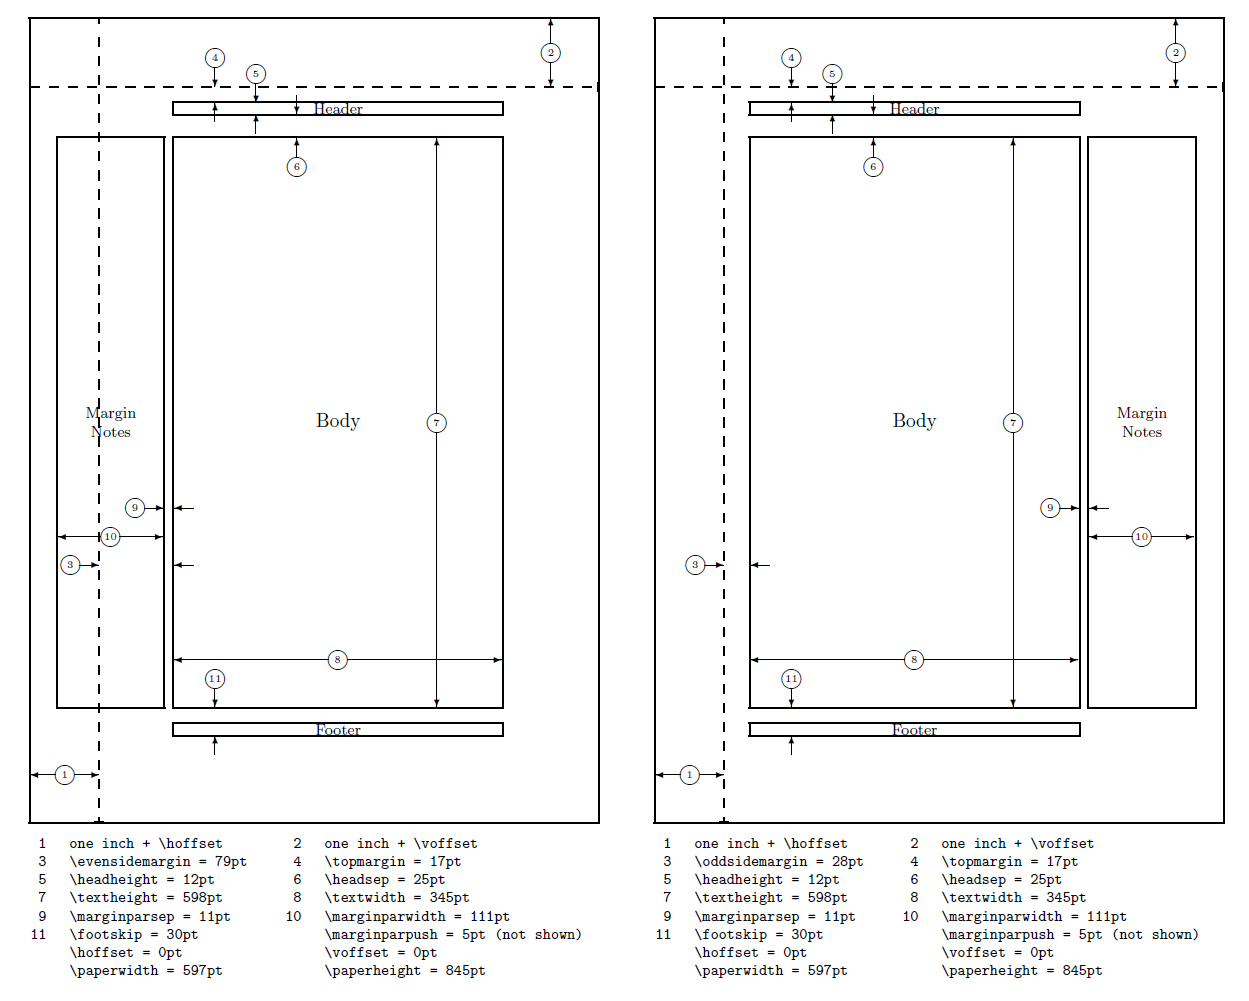
\includegraphics[width=0.75\textwidth]{images/layout.png}
\end{frame}

\begin{frame}{Alineando el texto}{Alineación de texto}
    \begin{columns}
        \column{0.5\textwidth}
            \begin{itemize}
                \item \textbf{Built-in}
                \begin{itemize}
                    \item \textbackslash raggedright
                    \item \textbackslash raggedleft
                    \item \textbackslash centering
                \end{itemize}
            \end{itemize}

        \pause
        
        \column{0.5\textwidth}
            \begin{itemize}
                \item \textbf{ragged2e}
                \begin{itemize}
                    \item \textbackslash Flush1Right
                    \item \textbackslash FlushLeft
                    \item \textbackslash Center
                    \item \textbackslash justify
                \end{itemize}
            \end{itemize}
    \end{columns}
\end{frame}